% Options for packages loaded elsewhere
\PassOptionsToPackage{unicode}{hyperref}
\PassOptionsToPackage{hyphens}{url}
%
\documentclass[
]{article}
\usepackage{amsmath,amssymb}
\usepackage{lmodern}
\usepackage{iftex}
\ifPDFTeX
  \usepackage[T1]{fontenc}
  \usepackage[utf8]{inputenc}
  \usepackage{textcomp} % provide euro and other symbols
\else % if luatex or xetex
  \usepackage{unicode-math}
  \defaultfontfeatures{Scale=MatchLowercase}
  \defaultfontfeatures[\rmfamily]{Ligatures=TeX,Scale=1}
\fi
% Use upquote if available, for straight quotes in verbatim environments
\IfFileExists{upquote.sty}{\usepackage{upquote}}{}
\IfFileExists{microtype.sty}{% use microtype if available
  \usepackage[]{microtype}
  \UseMicrotypeSet[protrusion]{basicmath} % disable protrusion for tt fonts
}{}
\makeatletter
\@ifundefined{KOMAClassName}{% if non-KOMA class
  \IfFileExists{parskip.sty}{%
    \usepackage{parskip}
  }{% else
    \setlength{\parindent}{0pt}
    \setlength{\parskip}{6pt plus 2pt minus 1pt}}
}{% if KOMA class
  \KOMAoptions{parskip=half}}
\makeatother
\usepackage{xcolor}
\usepackage[margin=1in]{geometry}
\usepackage{longtable,booktabs,array}
\usepackage{calc} % for calculating minipage widths
% Correct order of tables after \paragraph or \subparagraph
\usepackage{etoolbox}
\makeatletter
\patchcmd\longtable{\par}{\if@noskipsec\mbox{}\fi\par}{}{}
\makeatother
% Allow footnotes in longtable head/foot
\IfFileExists{footnotehyper.sty}{\usepackage{footnotehyper}}{\usepackage{footnote}}
\makesavenoteenv{longtable}
\usepackage{graphicx}
\makeatletter
\def\maxwidth{\ifdim\Gin@nat@width>\linewidth\linewidth\else\Gin@nat@width\fi}
\def\maxheight{\ifdim\Gin@nat@height>\textheight\textheight\else\Gin@nat@height\fi}
\makeatother
% Scale images if necessary, so that they will not overflow the page
% margins by default, and it is still possible to overwrite the defaults
% using explicit options in \includegraphics[width, height, ...]{}
\setkeys{Gin}{width=\maxwidth,height=\maxheight,keepaspectratio}
% Set default figure placement to htbp
\makeatletter
\def\fps@figure{htbp}
\makeatother
\setlength{\emergencystretch}{3em} % prevent overfull lines
\providecommand{\tightlist}{%
  \setlength{\itemsep}{0pt}\setlength{\parskip}{0pt}}
\setcounter{secnumdepth}{5}
\newlength{\cslhangindent}
\setlength{\cslhangindent}{1.5em}
\newlength{\csllabelwidth}
\setlength{\csllabelwidth}{3em}
\newlength{\cslentryspacingunit} % times entry-spacing
\setlength{\cslentryspacingunit}{\parskip}
\newenvironment{CSLReferences}[2] % #1 hanging-ident, #2 entry spacing
 {% don't indent paragraphs
  \setlength{\parindent}{0pt}
  % turn on hanging indent if param 1 is 1
  \ifodd #1
  \let\oldpar\par
  \def\par{\hangindent=\cslhangindent\oldpar}
  \fi
  % set entry spacing
  \setlength{\parskip}{#2\cslentryspacingunit}
 }%
 {}
\usepackage{calc}
\newcommand{\CSLBlock}[1]{#1\hfill\break}
\newcommand{\CSLLeftMargin}[1]{\parbox[t]{\csllabelwidth}{#1}}
\newcommand{\CSLRightInline}[1]{\parbox[t]{\linewidth - \csllabelwidth}{#1}\break}
\newcommand{\CSLIndent}[1]{\hspace{\cslhangindent}#1}
\ifLuaTeX
  \usepackage{selnolig}  % disable illegal ligatures
\fi
\IfFileExists{bookmark.sty}{\usepackage{bookmark}}{\usepackage{hyperref}}
\IfFileExists{xurl.sty}{\usepackage{xurl}}{} % add URL line breaks if available
\urlstyle{same} % disable monospaced font for URLs
\hypersetup{
  pdftitle={Temporal Dynamics of Normalization Reweighting},
  hidelinks,
  pdfcreator={LaTeX via pandoc}}

\title{Temporal Dynamics of Normalization Reweighting}
\author{Daniel H. Baker, Daniela Marinova, Richard Aveyard, Lydia J. Hargreaves, Alice Renton,\\
Ruby Castellani, Phoebe Hall, Miriam Harmens, Georgia Holroyd, Beth Nicholson,\\
Emily L. Williams, Hannah M. Hobson \& Alex R. Wade}
\date{2022-09-30}

\begin{document}
\maketitle

\hypertarget{abstract}{%
\section{Abstract}\label{abstract}}

For decades, neural suppression in early visual cortex has been thought to be fixed. But recent work has challenged this assumption by showing that suppression can be \emph{reweighted} based on recent history; when pairs of stimuli are repeatedly presented together, suppression between them strengthens. Here we investigate the temporal dynamics of this process using a steady-state VEP paradigm that provides a time-resolved, direct index of suppression between pairs of stimuli flickering at different frequencies (5 and 7Hz). Our initial analysis of an existing EEG dataset (N=100) indicated that suppression increases substantially during the first 2-5 seconds of stimulus presentation (with some variation across stimulation frequency). We then collected new EEG data (N=100) replicating this finding for both monocular and dichoptic mask arrangements in a preregistered study designed to measure reweighting. A third experiment (N=20) used source localized MEG, and found that these effects are apparent in primary visual cortex (V1), consistent with results from neurophysiological work. Because long-standing theories propose inhibition/excitation differences in autism, we also compared reweighting between individuals with high vs low autistic traits, and with and without an autism diagnosis, across our 3 data sets (total N=220). We find no compelling differences in reweighting that are associated with autism. Our results support the normalization reweighting model, and indicate that for prolonged stimulation, increases in suppression occur on the order of 2-5 seconds after stimulus onset.

\hypertarget{introduction}{%
\section{Introduction}\label{introduction}}

Suppressive interactions between neurons are ubiquitous in the nervous system, and normalization (or gain control) processes are considered a canonical neuronal computation (Carandini and Heeger, 2011). Yet for decades the strength of suppression was treated as fixed, largely due to the observation that adapting to one stimulus does not decrease its suppressive potency (Foley and Chen, 1997; Freeman et al., 2002). This orthodoxy was recently challenged by a series of innovative studies showing that normalization can be `reweighted' by recent history (Aschner et al., 2018; Westrick et al., 2016; Yiltiz et al., 2020). Specifically, when pairs of stimuli are repeatedly presented together, their neural representations come to suppress each other more strongly. This suggests that, far from being fixed, normalization is a dynamic process that is continuously updated by the sensory environment. Here, our objectives were to determine if the timecourse of these changes can be measured non-invasively from the human brain, assess if they occur similarly in distinct suppressive pathways, and determine whether they differ across the population as a function of autistic traits.

Plastic changes within the visual system occur over multiple timescales (see Webster, 2015 for a recent review). In the retina, adaptation to complete darkness takes around 30 minutes (Lamb and Pugh, 2006), and has established physiological substrates (i.e.~the regeneration rate of chemicals in different photoreceptor classes). Cortical forms of adaptation to cues such as stimulus contrast (Blakemore and Campbell, 1969), orientation (Gibson and Radner, 1937) and motion (Mather et al., 2008) can be observed within a few seconds, but also build up over durations on the order of several minutes (Greenlee et al., 1991). A recent form of binocular plasticity (Lunghi et al., 2011), in which one eye is patched and subsequently contributes more to binocular vision, requires more than an hour. Other types of adaptation have been identified with changes occurring over longer time periods, such as over several hours (Kwon et al., 2009) or days (Haak et al., 2014). Finally adaptation to specific combinations of orientation and colour (the McCollough, 1965 effect) can persist for several weeks (Jones and Holding, 1975), even with a brief induction period. Previous work on normalization reweighting has involved adapting sequences of around 40 -- 60s (Aschner et al., 2018; Yiltiz et al., 2020), though it is possible that reweighting might occur faster than this, consistent with other types of contrast adaptation.

Normalization itself is not a single process. Multiple suppressive pathways have been identified in the visual system, including between stimuli differing in orientation (Foley, 1994; Heeger, 1992), eye-of-origin (Legge, 1979; Sengpiel and Blakemore, 1994) and spatial position (Cannon and Fullenkamp, 1991; Petrov, 2005). At present there is evidence of normalization reweighting between stimuli with orthogonal orientations (Aschner et al., 2018), and adjacent spatial positions (Yiltiz et al., 2020). We anticipated that interocular suppression should also be subject to reweighting, but that there might be differences in the dynamics across suppressive pathways. This is plausible, given that suppression within and between the eyes has different spatiotemporal tuning (Meese and Baker, 2009), and dichoptic masking can be reduced by adapting to the mask (Baker et al., 2007; Li et al., 2005; Sengpiel and Vorobyov, 2005), unlike within-eye masking. Dynamic fluctuations in interocular suppression are a key feature of binocular rivalry (Alais et al., 2010; Wilson, 2003), for which autism-related differences have also been reported (Robertson et al., 2013). By comparing monocular and dichoptic suppression, we are also able to isolate any contribution of early pre-cortical factors. This is because interocular suppression impacts in primary visual cortex, and therefore bypasses earlier retinal and subcortical stages of processing that may contribute to monocular suppression (Li et al., 2005).

Atypical sensory experience is widely reported by individuals on the autism spectrum (MacLennan et al., 2022; Simmons et al., 2009), but the causal mechanisms remain unclear. Typical issues include hypersensitivity to intense stimuli such as loud sounds, bright lights and strong odours or flavours. Yet fundamental measures of sensitivity such as visual acuity (Tavassoli et al., 2011), contrast sensitivity (Koh et al., 2010), and audiometric performance (Rosenhall et al., 1999) are not consistently different from neurotypical controls. Theoretical accounts of sensory differences in autism have long proposed that the balance of inhibition and excitation may be disrupted (Rosenberg et al., 2015; Rubenstein and Merzenich, 2003), and there are isolated results that appear consistent with this. For example neural measures of surround suppression are weaker in autism (Schallmo et al., 2020), binocular rivalry is slower (Robertson et al., 2013) and orientation discrimination performance is better (Dickinson et al., 2014). Conversely, other studies have failed to find group differences using paradigms that should be equally dependent on inhibition, such as orientation repulsion (Van de Cruys et al., 2018), repetition suppression (Utzerath et al., 2018) and psychophysical measures of surround suppression (Sandhu et al., 2020). The evidence for atypical inhibition in autism is therefore currently inconclusive.

Our recent work has identified a potential autism-related difference in gain control using steady-state EEG methods. Vilidaite et al. (2018) measured contrast response functions for flickering stimuli in a large group of neurotypical adults, who were grouped according to their autism quotient (AQ, see Baron-Cohen et al., 2001) score. The responses were comparable between high and low AQ groups at the flicker frequency of the stimulus. However at the second harmonic frequency (twice the flicker frequency), the high AQ group showed weaker responses than the low AQ group. This effect was replicated in an independent sample of 12 adults with an autism diagnosis (compared with neurotypical controls). Because second harmonic responses are caused by nonlinear interactions in the visual system (they are absent in a linear system), and divisive suppression is a nonlinearity, this potentially implicates differences in suppression in autism. Furthermore, there appears to be a developmental trajectory, as autistic children tested as part of the same study (Vilidaite et al., 2018) showed weaker responses at both the first and second harmonic frequencies.

In this paper we perform a time-course analysis of a previously published EEG data set, and report two novel pre-registered experiments using EEG and MEG. Our data show that suppression increases substantially during the first 2-5 seconds following stimulus onset, for both monocular and dichoptic masks. Source localisation of MEG data indicate that the reweighting is present as early as primary visual cortex (V1). We also hypothesised that normalization reweighting might differ as a function of autistic traits. The relative novelty of the reweighting framework could explain why any differences have not previously been detected, and why the literature on inhibition in autism is relatively inconclusive. However we did not find convincing support for this hypothesis.

\hypertarget{results}{%
\section{Results}\label{results}}

We began by reanalysing data from a steady-state visually evoked potential (SSVEP) experiment reported by Vilidaite et al. (2018). Participants viewed arrays of flickering gratings of varying contrasts. In some conditions a single grating orientation was present flickering at 7Hz, whereas in other conditions a high contrast `mask' was added at right angles to the target gratings, and flickering at 5Hz. The left panel of Figure \ref{fig:Pilotdata}a shows contrast response functions with and without the mask - the presence of the mask reduces the 7Hz response to the target (blue squares are below the black circles; significant main effect of mask contrast, F(1,99) = 26.52, \emph{p} \textless{} 0.001). Similarly, the right panel of Figure \ref{fig:Pilotdata}a shows that the 5Hz response to the mask was itself suppressed by the presence of high contrast targets (main effect of target contrast on the mask response, F(2.92,288.63) = 46.77, \emph{p} \textless{} 0.001; note that the data from the masking conditions were not reported by Vilidaite et al. (2018)). At both frequencies, responses were localised to the occipital pole (see insets).

\begin{figure}

{\centering 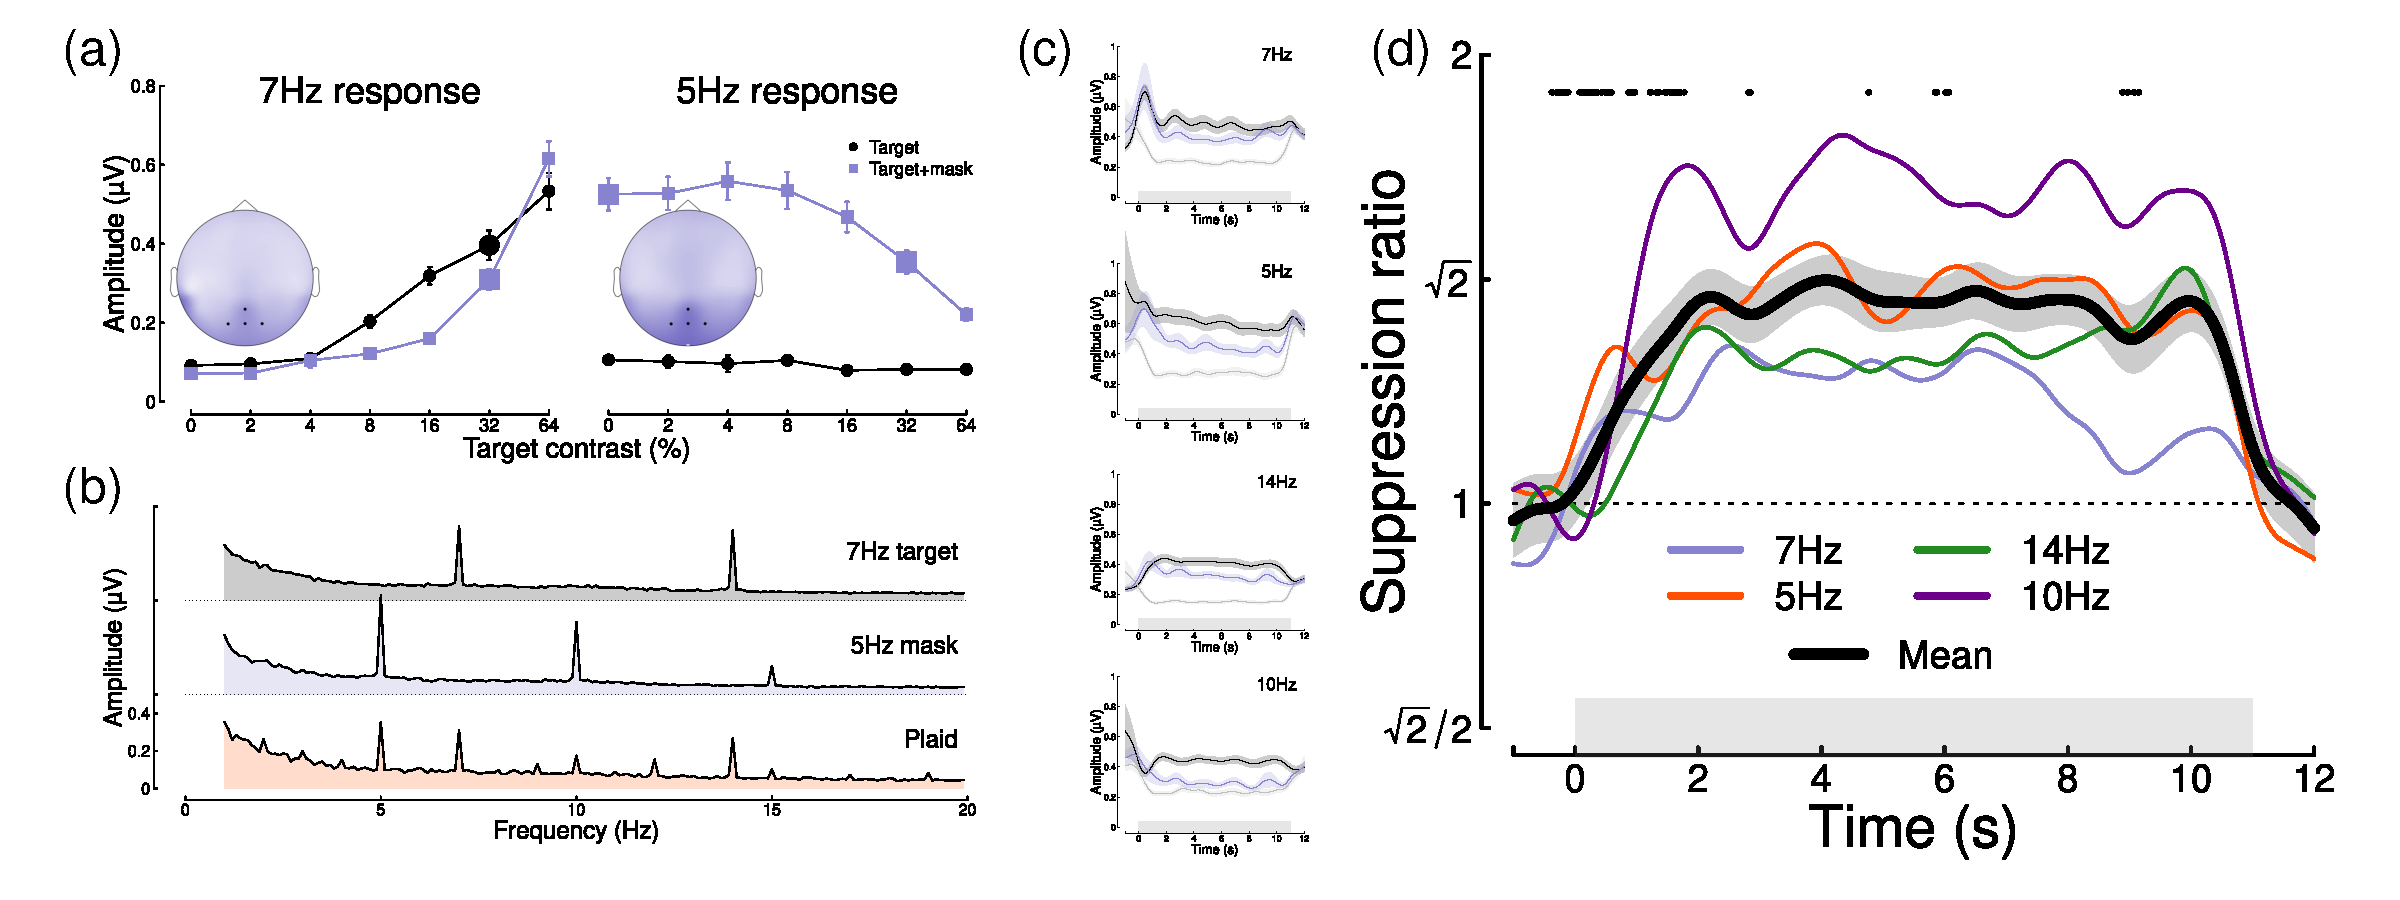
\includegraphics{Figures/VilidaiteData} 

}

\caption{Summary of pilot analysis of data from Vilidiate et al. (2018). Panel (a) shows contrast response functions at the target frequency (7Hz, left) and the mask frequency (5Hz, right). Insets show the distribution of activity across the scalp, with points marking the electrodes over which signals were averaged (Oz, POz, O1 and O2). Panel (b) shows Fourier spectra for the single component stimuli and their combination (plaid). Note the strong second harmonic components at 14Hz and 10Hz. Panel (c) shows timecourses of frequency-locked responses to a single stimulus (black) and the plaid stimulus (blue), compared to baseline (grey). Panel (d) shows the timecourse of suppression at each frequency (7Hz, 5Hz, 14Hz, 10Hz) and their average (black curve). Points around y = 1.8 indicate a significantly increasing ratio. Error bars in panel (a) and shaded regions in panels (c,d) indicate ±1SE across N=100 participants, and grey rectangles indicate the timing of stimulus presentation. The larger symbols in panel (a) indicate the conditions used for subsequent analyses.}\label{fig:Pilotdata}
\end{figure}

We then performed a timecourse analysis, in which we analysed each 11-second trial using a sliding 1-second time window. The top panel of Figure \ref{fig:Pilotdata}c shows the response at the target frequency (7Hz) to a single stimulus of 32\% contrast (black), and the response at 7Hz when the 32\% contrast mask is added (blue). Analogous responses are shown at three other frequencies - the mask frequency (5Hz), and the second harmonics of both target and mask frequencies (14Hz, 10Hz), at which strong responses were also found (see spectra in Figure \ref{fig:Pilotdata}b). The reduction in signal strength when the mask component is added illustrates the masking effect.

Taking the ratio of the two timecourses to calculate a masking index reveals that at 7Hz masking increases steeply during the first two seconds of stimulus presentation, and then plateaus for several seconds (blue trace in Figure \ref{fig:Pilotdata}d). A similar pattern is observed at 5Hz (red trace in Figure \ref{fig:Pilotdata}d), as well as at the second harmonics, with some variability in the timecourse across frequencies; for example at 5Hz suppression peaks at around 4 seconds. The black trace shows the average masking ratio across all four frequencies, which rises steeply for just over two seconds and then stays approximately constant until stimulus offset. We conducted cluster-corrected t-tests between ratios separated by 1000ms, testing for an increase in suppression ratio across time (i.e.~a one-sided test). Points at y = 1.8 in Figure \ref{fig:Pilotdata}d indicate time points where the ratio is significantly increasing, and occur mostly during the first 2 seconds of stimulus presentation.

Our initial reanalysis was promising, however the data were noisy despite the large sample size (of N=100), because each participant contributed only 8 trials (88 seconds) to each condition. We therefore preregistered two new experiments (see \url{https://osf.io/4qudc}) to investigate these effects in greater detail. These had a similar overall design to the Vilidaite et al. (2018) study, with some small changes intended to optimise the study (see Methods). The key differences were that we used shorter trials (because there were few changes in the latter part of the trials shown in Figure \ref{fig:Pilotdata}d), and also focussed all trials into a smaller number of conditions, such that each participant contributed 48 repetitions (288 seconds of data) to each of 4 conditions.

Figure \ref{fig:EEGdata} summarises the results of our EEG experiment testing a further 100 adult participants. Averaged EEG waveforms showed a strong oscillatory component at each of the two stimulus flicker frequencies (Figure \ref{fig:EEGdata}a), which slightly lagged the driving signal. Signals were well-isolated in the Fourier domain (Figure \ref{fig:EEGdata}b), and localised to occipital electrodes. Responses at 7Hz were weaker in the two masking conditions, showing significant changes in response amplitude for both the monocular (\emph{t} = 7.56, \emph{df} = 87, \emph{p} \textless{} 0.001) and dichoptic (\emph{t} = 11.35, \emph{df} = 87, \emph{p} \textless{} 0.001) masks. Dichoptic masking was significantly stronger than monocular masking (\emph{t} = 7.96, \emph{df} = 87, \emph{p} \textless{} 0.001), and a similar pattern was evident at 5Hz.

\begin{figure}

{\centering \includegraphics{temp/figures/Fig2} 

}

\caption{Summary of EEG results for N=100 adult participants. Panel (a) shows scalp topographies and averaged waveforms for 5Hz (top) and 7Hz (bottom) stimuli. The black sine wave trace in each panel illustrates the driving contrast modulation, and black points on the scalp topographies indicate electrodes Oz, O1, O2 and POz. Panel (b) shows the Fourier amplitude spectrum for each condition, with clear peaks at 5Hz and 7Hz. Panels (c,d) show timecourses at each frequency for the baseline condition (black), and the monocular (blue) and dichoptic (red) masking conditions. Panels (e,f) show suppression ratios as a function of time for each mask type, with points around y = 0.8 indicating a significantly increasing ratio. Shaded regions in panels (c-f) span ±1SE across participants, and light grey rectangles indicate the period of stimulus presentation.}\label{fig:EEGdata}
\end{figure}

The timecourse at both flicker frequencies showed an initial onset transient, and was then relatively stable for the 6 seconds of stimulus presentation (Figure \ref{fig:EEGdata}c,d). The ratio of target only to target + mask conditions increased over time (Figure \ref{fig:EEGdata}e,f) for both mask types. At 5Hz the increase in masking continued over the first 5 seconds of stimulus presentation (Figure \ref{fig:EEGdata}e; points at y = 0.8 indicate significantly increasing suppression), whereas at 7Hz the increase occurred primarily during the first second after onset (Figure \ref{fig:EEGdata}f). These differences across frequency are consistent with the pilot data (see Figure \ref{fig:Pilotdata}d). Both monocular and dichoptic masks produced similar timecourses of suppression. Overall, this second study confirmed that normalization increases during the first few seconds of a steady-state trial, and extends this finding to dichoptic mask arrangements.

\begin{figure}

{\centering \includegraphics{temp/figures/Fig3} 

}

\caption{Summary of MEG results for N=20 adults. Panel (a) shows average SSVEP response in source space, thresholded at SNR=2 (blue, left), and locations of the V1 ROI on the medial surface of both hemispheres (right, red). Panel (b) shows the Fourier spectra for the four experimental conditions, from the most responsive vertex in V1. Panels (c,d) show timecourses at 5Hz and 7Hz, and panels (e,f) show suppression ratios for the monocular and dichoptic conditions at each frequency, with points around y = 0.8 indicating a significantly increasing ratio. Shaded regions in panels (c-f) indicate ±1SE across participants, and light grey rectangles indicate the period of stimulus presentation.}\label{fig:MEGdata}
\end{figure}

Next we repeated the experiment on 20 participants using a 248-channel whole-head cryogenic MEG system. Half of the participants had a diagnosis of autism, and the remainder were age- and gender-matched controls. Source localisation using a linearly constrained minimum variance (LCMV) beamformer algorithm (Van Veen et al., 1997) showed strong localisation of steady-state signals at the occipital pole (see Figure \ref{fig:MEGdata}a), and in the Fourier domain (Figure \ref{fig:MEGdata}b). Responses from the most responsive V1 vertex showed a similar timecourse to those of the EEG experiments at both frequencies (Figure \ref{fig:MEGdata}c,d), and showed increasing suppression during the first few seconds of stimulus presentation (Figure \ref{fig:MEGdata}e,f). The normalization reweighting effect was again clearest at 5Hz, especially for the dichoptic condition (red curve in Figure \ref{fig:MEGdata}e). This confirms that the reweighting effects can occur as early as primary visual cortex, consistent with findings from neurophysiology (Aschner et al., 2018). However the data are more variable than for our EEG experiments, and had fewer significant clusters, owing to the smaller sample size for this dataset.

\begin{figure}

{\centering \includegraphics{temp/figures/Fig4} 

}

\caption{Analysis of the effect of autistic traits on normalization reweighting. Panels (a-c) show distributions of AQ scores across the three data sets. Panels (d-h) show timecourses of suppression averaged across stimulation frequency, and split by AQ score (d-f) or autism status (g, h). Panels (d,e,g) are for binocular or monocular presentation, and panels (f,h) are for dichoptic presentation. Shaded regions in panels (d-h) indicate ±1SE across participants, and black points at y = 0.8 indicate significant differences between groups.}\label{fig:AQanalysis}
\end{figure}

To investigate whether normalization reweighting effects differ with respect to autistic traits, we then split each dataset (averaged across temporal frequency) using median AQ score (for the EEG experiments) or according to diagnostic group (autism vs controls) for the MEG data. Figure \ref{fig:AQanalysis}a-c shows distributions of AQ scores for each experiment, and indicates for the pilot and EEG data which participants were in the high (purple) and low (green) AQ groups. The median AQ scores were 14 for the pilot data, and 18 for the EEG data, consistent with previous results for the general population (Baron-Cohen et al., 2001). In the MEG experiment, AQ scores for the autism group (mean 36.1) and the control group (mean 16.7) were significantly different (\emph{t} = 6.00, \emph{df} = 14.2, \emph{p} \textless{} 0.001), with minimal overlap (one participant with an autism diagnosis had an AQ score marginally lower than the highest AQ scores from the control group).

We compared the timecourse of suppression between groups using a nonparametric cluster correction approach (Maris and Oostenveld, 2007) to control the type I error rate. Significant clusters are indicated at y = 0.8 in panels d-h of Figure \ref{fig:AQanalysis}. Despite some occasionally significant clusters, there is no clear or consistent difference between groups across our three data sets. In particular, none of the significant clusters occur during the first few seconds of stimulus onset, when reweighting takes place. We also compared suppression ratios calculated on Fourier components for the full trial, and found no significant effects of autism on suppression strength. We therefore conclude that autism/AQ score is not associated with normalization reweighting, or the strength of suppression more generally.

\hypertarget{discussion}{%
\section{Discussion}\label{discussion}}

We found evidence of dynamic normalization reweighting across three separate datasets. Suppression increased significantly during the first 2-5 seconds of stimulus presentation, though with some variation across temporal frequency. Reweighting had a similar timecourse for monocular and dichoptic stimulus presentation, and was apparent as early as V1. We did not find compelling differences associated with autism, or high vs low autistic traits. In the remainder of this section we will discuss possible explanations for temporal frequency differences, evidence for inhibitory differences in autism, and more general implications of dynamic normalization reweighting.

One important question is whether the dynamic increase in suppression can be explained by the stimulus onset transient. This is a possibility that cannot be ruled out for some of our data. For example, the steep increase in suppression in Figure \ref{fig:EEGdata}f has a similar timecourse to the onset transient in Figure \ref{fig:EEGdata}d.~However, there are also counterexamples where suppression continues to increase well beyond the first 1 second of stimulus presentation (e.g.~Figure \ref{fig:EEGdata}e). It is currently unclear why there appear to be such substantial differences between temporal frequency conditions, especially with such similar frequencies (5 and 7Hz). However the differences are relatively consistent across experiments. For example, 5Hz flicker produces a more gradual increase in suppression across all three data sets, compared with 7Hz flicker. These differences may be a consequence of visual channels with different temporal tuning interacting with the stimulation frequency, as well as any nonlinearities that govern suppression. Or there could be an asymmetry, whereby the relative temporal frequency between the two stimulus components affects the character of suppression (Liza and Ray, 2022). We hope to be able to model these effects in the future, for example by using dynamic models of early vision that incorporate time-lagged gain control (e.g. Zhou et al., 2019).

We did not observe clear differences in the timecourse between monocular and dichoptic suppression. This is important, because the dichoptic arrangement bypasses early stages of processing before the cortex (e.g.~the retina and lateral geniculate nucleus). It suggests that the dynamic increases in suppression occur in the cortex, consistent with our MEG data that find evidence of reweighting in V1 (see Fig \ref{fig:MEGdata}), and with previous neurophysiological work (Aschner et al., 2018). It is currently unclear whether these effects originate in V1, or might involve feedback from higher areas. The similarity between monocular and dichoptic effects also differs from work on adaptation to individual mask components. In both physiological (Li et al., 2005; \textbf{Sengpiel2006?}) and psychophysical (Baker et al., 2007) paradigms, adapting to a dichoptic mask reduces its potency, whereas adapting to a monocular mask has little or no effect. Normalization reweighting offers an explanation for why monocular masks presented in isolation do not adapt: if suppressive weights are determined by co-occurrence of stimuli, presentation of an isolated mask will have little effect. However this cannot explain the dichoptic adaptation effects without invoking additional binocular processes, such as competition between summing and differencing channels (e.g. May et al., 2012).

The relationship between normalization reweighting and other forms of visual plasticity is currently unclear. One phenomenon that might be closely related to our dichoptic effect is the change in interocular suppression that occurs when one eye is patched for a period of time (Lunghi et al., 2011). In the patching paradigm, the inputs to the two eyes are uncorrelated while one eye is patched, which the normalization reweighting model predicts should reduce suppression between the eyes. Most studies using patching have focussed on the resulting imbalance between the patched and non-patched eye, in which the patched eye contributes more to binocular single vision than the non-patched eye. In principle this could be due to increased suppression of the non-patched eye (inconsistent with normalization reweighting), or reduced suppression of the patched eye (consistent with normalization reweighting). It is difficult to distinguish these possibilities using paradigms that assess the balance between the two eyes, such as the binocular rivalry paradigm from the original Lunghi et al. (2011) study. However subsequent work has shown that patching increases the patched eye's response (Zhou et al., 2015), and reduces both dichoptic masking (Baldwin and Hess, 2018) and levels of the inhibitory neurotransmitter GABA (Lunghi et al., 2015). All of these findings are consistent with a reweighting account.

Participants in Experiments 2 \& 3 also completed the sensory perception quotient (SPQ) scale. SPQ scores showed significant negative correlation with AQ for both data sets (EEG data, \emph{r} = -0.35, \emph{p} \textless{} 0.001; MEG data, \emph{r} = -0.57, \emph{p} = 0.011) with effect sizes comparable to those reported previously (Tavassoli et al., 2014). We also conducted an exploratory analysis of the EEG data from Experiment 2, splitting participants by SPQ instead of AQ. However this analysis did not reveal any convincing differences in normalization reweighting either. Our preregistration also proposed to replicate our earlier finding of a reduced second harmonic response in participants with autism/high AQ scores. However the changes to the experimental design greatly reduced the second harmonic response in both experiments, such that it could not be observed reliably (see Figures \ref{fig:EEGdata}b and \ref{fig:MEGdata}b). We were therefore not confident in conducting this analysis. We suspect that the increase in spatial frequency from 0.5 c/deg in the Vilidaite et al. (2018) study to 2 c/deg here is most likely responsible for the dramatically reduced second harmonic response.

The idea that the dynamic balance of inhibition and excitation might be different in autism (Rosenberg et al., 2015; Rubenstein and Merzenich, 2003) has compelling face validity. For example individuals with autism often report difficulties with changes in their sensory environment, which might be due to gain control processes failing to adapt appropriately. Indeed, there is experimental evidence of reduced adaptation across various domains (Pellicano et al., 2007; Turi et al., 2015), which is predicted by some autism models (Pellicano and Burr, 2012). However this appears not to extend to changes in normalization reweighting, despite the link between reweighting and adaptation (Westrick et al., 2016).

\hypertarget{conclusions}{%
\subsection{Conclusions}\label{conclusions}}

We investigated the timecourse of normalization reweighting across three datasets, with a total of 220 participants. We found clear evidence that suppression increases during the first 2-5 seconds of stimulus presentation, though there were differences across frequency that are currently unexplained. We did not find evidence of autism-related differences in either the magnitude or timecourse of suppression. Our results support an emerging theory that suppression is a dynamic process that allows sensory systems to recalibrate according to their recent history.

\hypertarget{methods}{%
\section{Methods}\label{methods}}

\hypertarget{participants}{%
\subsection{Participants}\label{participants}}

Experiment 1 was completed by 100 adult participants (32 male, 68 female; mean age 21.9) in early 2015, and first reported by Vilidaite et al. (2018). Here we reanalysed the dataset, and report the results of masking conditions not previously published. Experiment 2 was completed by 100 adult participants (23 male, 74 female, 3 other/not stated; mean age 22.1) in early 2022. Experiment 3 was completed by 10 adults (2 male, 8 female) with a clinical diagnosis of autism, and 10 control participants who were closely matched for age (means of 21.8 and 22, \emph{t} = 0.18, \emph{df} = 18, \emph{p} = 0.86) and exactly matched for gender. Procedures in Experiments 1 and 2 were approved by the ethics committee of the Department of Psychology at the University of York. Procedures for Experiment 3 were approved by the ethics committee of the York Neuroimaging Centre. All participants provided written informed consent.

\hypertarget{apparatus-and-stimuli}{%
\subsection{Apparatus and stimuli}\label{apparatus-and-stimuli}}

In Experiments 1 and 2, stimuli were presented using a ViewPixx 3D LCD display device (VPixx Technologies, Canada) with a resolution of 1920 \(\times\) 1080 pixels and a refresh rate of 120Hz. The display was gamma corrected using a Minolta LS110 photometer. In Experiment 2, participants wore active stereo shutter glasses (NVidia 3D Vision 2) that were synchronised with the display using an infra-red signal. EEG data were collected using a 64-channel Waveguard cap, and were amplified and digitised at 1000Hz using an ANT Neuroscan system. Electrode impedance was maintained below 5k\(\Omega\), and referenced to a whole-head average.

In Experiment 3, stimuli were presented using a ProPixx DLP projector (VPixx Technologies) running at 120Hz. Stereo presentation was enabled using a circular polariser that was synchronised with the projector refresh, and participants wore passive polarised glasses during the experiment. DLP projectors are perfectly linear, so gamma correction was not required. Data were acquired using a refurbished 248-channel 4D Neuroimaging Magnes 3600 MEG scanner, recording at 1001Hz. Participant head shape was digitised using a Polhemus Fastrak device, and head position was recorded at the start and end of each block by passing current through 5 position coils placed at fiducial points on the head. We also obtained structural MRI scans using a 3 Tesla Siemens Magnetom Prisma scanner to aid in source localisation. Two participants were not available for MRI scans, so we used the MNI ICBM152 template brain (Fonov et al., 2011) for these individuals.

Stimuli were patches of sine wave grating with a diameter of 2 degrees, flickering sinusoidally (on/off flicker) at either 5Hz or 7Hz. In Experiment 1 the gratings had a spatial frequency of 0.5c/deg, and in Experiments 2 \& 3 this was increased to 2c/deg. A symmetrical array of 36 individual patches tiled the display. In Experiment 1 the patch orientation was randomly selected on each trial, and all patches had the same orientation. In Experiments 2 \& 3 each patch had a random orientation, which was intended to prevent any sequential effects between trials with similar orientations. The central patch was omitted and replaced by a fixation marker constructed from randomly overlaid squares. During each experiment, the fixation marker could be resampled on each trial with a probability of 0.5. Participants were instructed to monitor the fixation marker and count the number of times it changed throughout the experiment. This was intended to maintain attention towards the display and keep participants occupied.

Participants also completed either the short AQ (Hoekstra et al., 2011) in Experiment 1, or the full AQ (Baron-Cohen et al., 2001) in Experiments 2 and 3. For comparison across experiments, we rescaled the short AQ to the same range as the full AQ (0-50). In Experiments 2 and 3, the sensory perception quotient (SPQ) questionnaire (Tavassoli et al., 2014) was also completed.

\hypertarget{procedures}{%
\subsection{Procedures}\label{procedures}}

In Experiment 1, target stimuli flickering at 7Hz were presented at a range of contrasts (1 - 64\%). In half of the conditions a superimposed orthogonal mask of 32\% contrast was presented simultaneously, flickering at 5Hz. Stimuli were displayed for trials of 11 seconds, with a 3 second inter-trial interval. The experiment consisted of 4 blocks of trials, each lasting around 10 minutes, and resulting in 8 repetitions of each condition. Participants viewed the display from 57cm, were comfortably seated in an upright position, and were able to rest between blocks. Low latency 8-bit digital triggers transmitted the trial onset and condition information directly to the EEG amplifier.

The procedure for Experiment 2 was very similar, except that participants also wore stereo shutter glasses during the experiment. There were four conditions: (i) monocular presentation of a 5Hz stimulus of 48\% contrast, (ii) monocular presentation of a 7Hz stimulus of 48\% contrast, (iii) monocular presentation of both stimuli superimposed at right angles, and (iv) dichoptic presentation of both stimuli at right angles (i.e.~one stimulus to the left eye, one to the right eye). Eye of presentation was pseudo-randomised to ensure equal numbers of left-eye and right-eye presentations. The trial duration was 6 seconds, with a 3 second inter-trial interval. Participants completed 3 blocks, each lasting around 10 minutes, resulting in a total of 48 repetitions of each condition. Experiment 3 was identical, except that the projector screen was viewed from a distance of 85cm.

\hypertarget{data-analysis}{%
\subsection{Data analysis}\label{data-analysis}}

EEG data from Experiments 1 and 2 were first imported into Matlab using components of the EEGlab toolbox (Delorme and Makeig, 2004), and converted into a compressed ASCII format. Primary data analysis was then conducted using a bespoke \emph{R} script. In brief, we epoched each trial and extracted the average timecourse across four occipital electrodes (\emph{Oz}, \emph{POz}, \emph{O1} and \emph{O2}), and then calculated the Fourier transform of this average waveform. We excluded trials for which the Mahalanobis distance of the complex Fourier components exceeded 3 (for details see Baker, 2021). This resulted in 0.25\% of trials being excluded for Experiment 1, 4.51\% of trials for Experiment 2, and 4.51\% of trials for Experiment 3. Next we averaged the waveforms across all remaining trials, and calculated the Fourier transform in a 1-second sliding window to generate timecourses for each participant. We divided the timecourse for the target-only condition by the timecourse for the target + mask condition to produce a suppression ratio. These were then converted to logarithmic (dB) units for averaging, calculation of standard errors, and statistical comparisons. For display purposes we smoothed the timecourses using a cubic spline function, however all statistical comparisons used the unsmoothed data.

For Experiment 3, we performed source localisation using a linearly constrained minimum variance (LCMV) beamformer algorithm, implemented in Brainstorm (Tadel et al., 2011). Structural MRI scans were processed using Freesurfer (Dale et al., 1999) to generate a 3D mesh of the head and brain, and we calculated source weights for each block with reference to a 5-minute empty room recording, usually recorded on the day of the experiment. The matrix of source weights for each block was used in a custom Matlab script to extract signals from V1, identified using the probabilistic maps of Wang et al. (2015). These signals were then imported into R for the main analysis, which was consistent with the EEG analysis described above.

To make comparisons between groups of participants across time, we used a non-parametric cluster correction technique (Maris and Oostenveld, 2007) based on t-tests. Clusters were identified as temporally adjacent observations that were all statistically significant, and a summed t-value was calculated for each cluster. A null distribution was then generated by randomising group membership and recalculating the summed t-value for the largest cluster, and repeating this procedure 1000 times. Clusters were considered significant if they fell outside of the 95\% confidence limits of the null distribution. We adapted this approach to test for significantly increasing suppression by conducting one-way t-tests between time points separated by 1000ms, and repeating the cluster correction procedure as described above.

\hypertarget{preregistration-data-and-code-availability}{%
\subsection{Preregistration, data and code availability}\label{preregistration-data-and-code-availability}}

Following a preliminary analysis of the data from Experiment 1, we preregistered our hypotheses and analysis plan for Experiments 2 and 3 on the Open Science Framework website. The preregistration document, along with raw and processed data, and analysis scripts, are publicly available at the project repository: \url{https://osf.io/ab3yv/}

\hypertarget{acknowledgements}{%
\section{Acknowledgements}\label{acknowledgements}}

Supported by BBSRC grant BB/V007580/1 awarded to DHB and ARW. We are grateful to all of the participants who took part in the experiments reported here.

\hypertarget{references}{%
\section*{References}\label{references}}
\addcontentsline{toc}{section}{References}

\hypertarget{refs}{}
\begin{CSLReferences}{1}{0}
\leavevmode\vadjust pre{\hypertarget{ref-Alais2010}{}}%
Alais D, Cass J, OShea RP, Blake R. 2010. Visual sensitivity underlying changes in visual consciousness. \emph{Current Biology} \textbf{20}:1362--1367. doi:\href{https://doi.org/10.1016/j.cub.2010.06.015}{10.1016/j.cub.2010.06.015}

\leavevmode\vadjust pre{\hypertarget{ref-Aschner2018}{}}%
Aschner A, Solomon SG, Landy MS, Heeger DJ, Kohn A. 2018. Temporal contingencies determine whether adaptation strengthens or weakens normalization. \emph{J Neurosci} \textbf{38}:10129--10142. doi:\href{https://doi.org/10.1523/JNEUROSCI.1131-18.2018}{10.1523/JNEUROSCI.1131-18.2018}

\leavevmode\vadjust pre{\hypertarget{ref-Baker2021}{}}%
Baker DH. 2021. Statistical analysis of periodic data in neuroscience. \emph{Neurons, Behavior, Data analysis, and Theory} \textbf{5}. doi:\href{https://doi.org/10.51628/001c.27680}{10.51628/001c.27680}

\leavevmode\vadjust pre{\hypertarget{ref-Baker2007}{}}%
Baker DH, Meese TS, Summers RJ. 2007. Psychophysical evidence for two routes to suppression before binocular summation of signals in human vision. \emph{Neuroscience} \textbf{146}:435--448. doi:\href{https://doi.org/10.1016/j.neuroscience.2007.01.030}{10.1016/j.neuroscience.2007.01.030}

\leavevmode\vadjust pre{\hypertarget{ref-Baldwin2018}{}}%
Baldwin AS, Hess RF. 2018. The mechanism of short-term monocular deprivation is not simple: Separate effects on parallel and cross-oriented dichoptic masking. \emph{Sci Rep} \textbf{8}:6191. doi:\href{https://doi.org/10.1038/s41598-018-24584-9}{10.1038/s41598-018-24584-9}

\leavevmode\vadjust pre{\hypertarget{ref-Baron-Cohen2001}{}}%
Baron-Cohen S, Wheelwright S, Skinner R, Martin J, Clubley E. 2001. The autism-spectrum quotient (AQ): Evidence from asperger syndrome/high-functioning autism, males and females, scientists and mathematicians. \emph{J Autism Dev Disord} \textbf{31}:5--17. doi:\href{https://doi.org/10.1023/a:1005653411471}{10.1023/a:1005653411471}

\leavevmode\vadjust pre{\hypertarget{ref-Blakemore1969}{}}%
Blakemore C, Campbell FW. 1969. On the existence of neurones in the human visual system selectively sensitive to the orientation and size of retinal images. \emph{J Physiol} \textbf{203}:237--60. doi:\href{https://doi.org/10.1113/jphysiol.1969.sp008862}{10.1113/jphysiol.1969.sp008862}

\leavevmode\vadjust pre{\hypertarget{ref-Cannon1991}{}}%
Cannon MW, Fullenkamp SC. 1991. Spatial interactions in apparent contrast: Inhibitory effects among grating patterns of different spatial frequencies, spatial positions and orientations. \emph{Vision Res} \textbf{31}:1985--98. doi:\href{https://doi.org/10.1016/0042-6989(91)90193-9}{10.1016/0042-6989(91)90193-9}

\leavevmode\vadjust pre{\hypertarget{ref-Carandini2011}{}}%
Carandini M, Heeger DJ. 2011. Normalization as a canonical neural computation. \emph{Nature Reviews Neuroscience} \textbf{13}:51--62. doi:\href{https://doi.org/10.1038/nrn3136}{10.1038/nrn3136}

\leavevmode\vadjust pre{\hypertarget{ref-Dale1999}{}}%
Dale AM, Fischl B, Sereno MI. 1999. Cortical surface-based analysis. I. Segmentation and surface reconstruction. \emph{Neuroimage} \textbf{9}:179--94. doi:\href{https://doi.org/10.1006/nimg.1998.0395}{10.1006/nimg.1998.0395}

\leavevmode\vadjust pre{\hypertarget{ref-Delorme2004}{}}%
Delorme A, Makeig S. 2004. EEGLAB: An open source toolbox for analysis of single-trial EEG dynamics including independent component analysis. \emph{J Neurosci Methods} \textbf{134}:9--21. doi:\href{https://doi.org/10.1016/j.jneumeth.2003.10.009}{10.1016/j.jneumeth.2003.10.009}

\leavevmode\vadjust pre{\hypertarget{ref-Dickinson2014}{}}%
Dickinson A, Jones M, Milne E. 2014. Oblique orientation discrimination thresholds are superior in those with a high level of autistic traits. \emph{Journal of Autism and Developmental Disorders} \textbf{44}:2844--2850. doi:\href{https://doi.org/10.1007/s10803-014-2147-1}{10.1007/s10803-014-2147-1}

\leavevmode\vadjust pre{\hypertarget{ref-Foley1994}{}}%
Foley JM. 1994. Human luminance pattern-vision mechanisms: Masking experiments require a new model. \emph{J Opt Soc Am A Opt Image Sci Vis} \textbf{11}:1710--9. doi:\href{https://doi.org/10.1364/josaa.11.001710}{10.1364/josaa.11.001710}

\leavevmode\vadjust pre{\hypertarget{ref-Foley1997}{}}%
Foley JM, Chen CC. 1997. Analysis of the effect of pattern adaptation on pattern pedestal effects: A two-process model. \emph{Vision Res} \textbf{37}:2779--88. doi:\href{https://doi.org/10.1016/s0042-6989(97)00081-3}{10.1016/s0042-6989(97)00081-3}

\leavevmode\vadjust pre{\hypertarget{ref-Fonov2011}{}}%
Fonov V, Evans AC, Botteron K, Almli CR, McKinstry RC, Collins DL, Brain Development Cooperative Group. 2011. Unbiased average age-appropriate atlases for pediatric studies. \emph{Neuroimage} \textbf{54}:313--27. doi:\href{https://doi.org/10.1016/j.neuroimage.2010.07.033}{10.1016/j.neuroimage.2010.07.033}

\leavevmode\vadjust pre{\hypertarget{ref-Freeman2002}{}}%
Freeman TCB, Durand S, Kiper DC, Carandini M. 2002. Suppression without inhibition in visual cortex. \emph{Neuron} \textbf{35}:759--71. doi:\href{https://doi.org/10.1016/s0896-6273(02)00819-x}{10.1016/s0896-6273(02)00819-x}

\leavevmode\vadjust pre{\hypertarget{ref-Gibson1937}{}}%
Gibson JJ, Radner M. 1937. Adaptation, after-effect and contrast in the perception of tilted lines. {I}. {Quantitative} studies. \emph{Journal of Experimental Psychology} \textbf{20}:453--467. doi:\href{https://doi.org/10.1037/h0059826}{10.1037/h0059826}

\leavevmode\vadjust pre{\hypertarget{ref-Greenlee1991}{}}%
Greenlee MW, Georgeson MA, Magnussen S, Harris JP. 1991. The time course of adaptation to spatial contrast. \emph{Vision Res} \textbf{31}:223--36. doi:\href{https://doi.org/10.1016/0042-6989(91)90113-j}{10.1016/0042-6989(91)90113-j}

\leavevmode\vadjust pre{\hypertarget{ref-Haak2014}{}}%
Haak KV, Fast E, Bao M, Lee M, Engel SA. 2014. Four days of visual contrast deprivation reveals limits of neuronal adaptation. \emph{Curr Biol} \textbf{24}:2575--9. doi:\href{https://doi.org/10.1016/j.cub.2014.09.027}{10.1016/j.cub.2014.09.027}

\leavevmode\vadjust pre{\hypertarget{ref-Heeger1992}{}}%
Heeger DJ. 1992. Normalization of cell responses in cat striate cortex. \emph{Vis Neurosci} \textbf{9}:181--97. doi:\href{https://doi.org/10.1017/s0952523800009640}{10.1017/s0952523800009640}

\leavevmode\vadjust pre{\hypertarget{ref-Hoekstra2011}{}}%
Hoekstra RA, Vinkhuyzen AAE, Wheelwright S, Bartels M, Boomsma DI, Baron-Cohen S, Posthuma D, Sluis S van der. 2011. The construction and validation of an abridged version of the autism-spectrum quotient (AQ-short). \emph{J Autism Dev Disord} \textbf{41}:589--96. doi:\href{https://doi.org/10.1007/s10803-010-1073-0}{10.1007/s10803-010-1073-0}

\leavevmode\vadjust pre{\hypertarget{ref-Jones1975}{}}%
Jones PD, Holding DH. 1975. Extremely long-term persistence of the McCollough effect. \emph{J Exp Psychol Hum Percept Perform} \textbf{1}:323--7. doi:\href{https://doi.org/10.1037//0096-1523.1.4.323}{10.1037//0096-1523.1.4.323}

\leavevmode\vadjust pre{\hypertarget{ref-Koh2010}{}}%
Koh HC, Milne E, Dobkins K. 2010. Spatial contrast sensitivity in adolescents with autism spectrum disorders. \emph{J Autism Dev Disord} \textbf{40}:978--87. doi:\href{https://doi.org/10.1007/s10803-010-0953-7}{10.1007/s10803-010-0953-7}

\leavevmode\vadjust pre{\hypertarget{ref-Kwon2009}{}}%
Kwon M, Legge GE, Fang F, Cheong AMY, He S. 2009. Adaptive changes in visual cortex following prolonged contrast reduction. \emph{J Vis} \textbf{9}:20.1--16. doi:\href{https://doi.org/10.1167/9.2.20}{10.1167/9.2.20}

\leavevmode\vadjust pre{\hypertarget{ref-Lamb2006}{}}%
Lamb TD, Pugh EN Jr. 2006. Phototransduction, dark adaptation, and rhodopsin regeneration the proctor lecture. \emph{Invest Ophthalmol Vis Sci} \textbf{47}:5137--52. doi:\href{https://doi.org/10.1167/iovs.06-0849}{10.1167/iovs.06-0849}

\leavevmode\vadjust pre{\hypertarget{ref-Legge1979}{}}%
Legge GE. 1979. Spatial frequency masking in human vision: Binocular interactions. \emph{J Opt Soc Am} \textbf{69}:838--47. doi:\href{https://doi.org/10.1364/josa.69.000838}{10.1364/josa.69.000838}

\leavevmode\vadjust pre{\hypertarget{ref-Li2005}{}}%
Li B, Peterson MR, Thompson JK, Duong T, Freeman RD. 2005. Cross-orientation suppression: Monoptic and dichoptic mechanisms are different. \emph{J Neurophysiol} \textbf{94}:1645--50. doi:\href{https://doi.org/10.1152/jn.00203.2005}{10.1152/jn.00203.2005}

\leavevmode\vadjust pre{\hypertarget{ref-Liza2022}{}}%
Liza K, Ray S. 2022. Local interactions between steady-state visually evoked potentials at nearby flickering frequencies. \emph{J Neurosci} \textbf{42}:3965--3974. doi:\href{https://doi.org/10.1523/JNEUROSCI.0180-22.2022}{10.1523/JNEUROSCI.0180-22.2022}

\leavevmode\vadjust pre{\hypertarget{ref-Lunghi2011}{}}%
Lunghi C, Burr DC, Morrone C. 2011. Brief periods of monocular deprivation disrupt ocular balance in human adult visual cortex. \emph{Curr Biol} \textbf{21}:R538--9. doi:\href{https://doi.org/10.1016/j.cub.2011.06.004}{10.1016/j.cub.2011.06.004}

\leavevmode\vadjust pre{\hypertarget{ref-Lunghi2015}{}}%
Lunghi C, Emir UE, Morrone MC, Bridge H. 2015. Short-term monocular deprivation alters GABA in the adult human visual cortex. \emph{Curr Biol} \textbf{25}:1496--501. doi:\href{https://doi.org/10.1016/j.cub.2015.04.021}{10.1016/j.cub.2015.04.021}

\leavevmode\vadjust pre{\hypertarget{ref-MacLennan2022}{}}%
MacLennan K, O'Brien S, Tavassoli T. 2022. In our own words: The complex sensory experiences of autistic adults. \emph{J Autism Dev Disord} \textbf{52}:3061--3075. doi:\href{https://doi.org/10.1007/s10803-021-05186-3}{10.1007/s10803-021-05186-3}

\leavevmode\vadjust pre{\hypertarget{ref-Maris2007}{}}%
Maris E, Oostenveld R. 2007. Nonparametric statistical testing of EEG- and MEG-data. \emph{J Neurosci Methods} \textbf{164}:177--90. doi:\href{https://doi.org/10.1016/j.jneumeth.2007.03.024}{10.1016/j.jneumeth.2007.03.024}

\leavevmode\vadjust pre{\hypertarget{ref-Mather2008}{}}%
Mather G, Pavan A, Campana G, Casco C. 2008. The motion aftereffect reloaded. \emph{Trends Cogn Sci} \textbf{12}:481--7. doi:\href{https://doi.org/10.1016/j.tics.2008.09.002}{10.1016/j.tics.2008.09.002}

\leavevmode\vadjust pre{\hypertarget{ref-May2012}{}}%
May KA, Zhaoping L, Hibbard PB. 2012. Perceived direction of motion determined by adaptation to static binocular images. \emph{Curr Biol} \textbf{22}:28--32. doi:\href{https://doi.org/10.1016/j.cub.2011.11.025}{10.1016/j.cub.2011.11.025}

\leavevmode\vadjust pre{\hypertarget{ref-McCollough1965}{}}%
McCollough C. 1965. Color adaptation of edge-detectors in the human visual system. \emph{Science} \textbf{149}:1115--6. doi:\href{https://doi.org/10.1126/science.149.3688.1115}{10.1126/science.149.3688.1115}

\leavevmode\vadjust pre{\hypertarget{ref-Meese2009}{}}%
Meese TS, Baker DH. 2009. Cross-orientation masking is speed invariant between ocular pathways but speed dependent within them. \emph{Journal of Vision} \textbf{9}:2. doi:\href{https://doi.org/10.1167/9.5.2}{10.1167/9.5.2}

\leavevmode\vadjust pre{\hypertarget{ref-Pellicano2012}{}}%
Pellicano E, Burr D. 2012. When the world becomes 'too real': A bayesian explanation of autistic perception. \emph{Trends Cogn Sci} \textbf{16}:504--10. doi:\href{https://doi.org/10.1016/j.tics.2012.08.009}{10.1016/j.tics.2012.08.009}

\leavevmode\vadjust pre{\hypertarget{ref-Pellicano2007}{}}%
Pellicano E, Jeffery L, Burr D, Rhodes G. 2007. Abnormal adaptive face-coding mechanisms in children with autism spectrum disorder. \emph{Curr Biol} \textbf{17}:1508--12. doi:\href{https://doi.org/10.1016/j.cub.2007.07.065}{10.1016/j.cub.2007.07.065}

\leavevmode\vadjust pre{\hypertarget{ref-Petrov2005}{}}%
Petrov Y. 2005. Two distinct mechanisms of suppression in human vision. \emph{Journal of Neuroscience} \textbf{25}:8704--8707. doi:\href{https://doi.org/10.1523/jneurosci.2871-05.2005}{10.1523/jneurosci.2871-05.2005}

\leavevmode\vadjust pre{\hypertarget{ref-Robertson2013}{}}%
Robertson CE, Kravitz DJ, Freyberg J, Baron-Cohen S, Baker CI. 2013. Slower rate of binocular rivalry in autism. \emph{The Journal of Neuroscience} \textbf{33}:16983--16991. doi:\href{https://doi.org/10.1523/jneurosci.0448-13.2013}{10.1523/jneurosci.0448-13.2013}

\leavevmode\vadjust pre{\hypertarget{ref-Rosenberg2015}{}}%
Rosenberg A, Patterson JS, Angelaki DE. 2015. A computational perspective on autism. \emph{Proc Natl Acad Sci U S A} \textbf{112}:9158--65. doi:\href{https://doi.org/10.1073/pnas.1510583112}{10.1073/pnas.1510583112}

\leavevmode\vadjust pre{\hypertarget{ref-Rosenhall1999}{}}%
Rosenhall U, Nordin V, Sandström M, Ahlsén G, Gillberg C. 1999. Autism and hearing loss. \emph{J Autism Dev Disord} \textbf{29}:349--57. doi:\href{https://doi.org/10.1023/a:1023022709710}{10.1023/a:1023022709710}

\leavevmode\vadjust pre{\hypertarget{ref-Rubenstein2003}{}}%
Rubenstein JLR, Merzenich MM. 2003. Model of autism: Increased ratio of excitation/inhibition in key neural systems. \emph{Genes Brain Behav} \textbf{2}:255--67. doi:\href{https://doi.org/10.1034/j.1601-183x.2003.00037.x}{10.1034/j.1601-183x.2003.00037.x}

\leavevmode\vadjust pre{\hypertarget{ref-Sandhu2020}{}}%
Sandhu TR, Reese G, Lawson RP. 2020. Preserved low-level visual gain control in autistic adults. \emph{Wellcome Open Research} \textbf{4}. doi:\href{https://doi.org/10.12688/wellcomeopenres.15615.1}{10.12688/wellcomeopenres.15615.1}

\leavevmode\vadjust pre{\hypertarget{ref-Schallmo2020}{}}%
Schallmo M-P, Kolodny T, Kale AM, Millin R, Flevaris AV, Edden RAE, Gerdts J, Bernier RA, Murray SO. 2020. Weaker neural suppression in autism. \emph{Nat Commun} \textbf{11}:2675. doi:\href{https://doi.org/10.1038/s41467-020-16495-z}{10.1038/s41467-020-16495-z}

\leavevmode\vadjust pre{\hypertarget{ref-Sengpiel1994}{}}%
Sengpiel F, Blakemore C. 1994. Interocular control of neuronal responsiveness in cat visual cortex. \emph{Nature} \textbf{368}:847--50. doi:\href{https://doi.org/10.1038/368847a0}{10.1038/368847a0}

\leavevmode\vadjust pre{\hypertarget{ref-Sengpiel2005}{}}%
Sengpiel F, Vorobyov V. 2005. Intracortical origins of interocular suppression in the visual cortex. \emph{J Neurosci} \textbf{25}:6394--400. doi:\href{https://doi.org/10.1523/JNEUROSCI.0862-05.2005}{10.1523/JNEUROSCI.0862-05.2005}

\leavevmode\vadjust pre{\hypertarget{ref-Simmons2009}{}}%
Simmons DR, Robertson AE, McKay LS, Toal E, McAleer P, Pollick FE. 2009. Vision in autism spectrum disorders. \emph{Vision Research} \textbf{49}:2705--2739. doi:\href{https://doi.org/10.1016/j.visres.2009.08.005}{10.1016/j.visres.2009.08.005}

\leavevmode\vadjust pre{\hypertarget{ref-Tadel2011}{}}%
Tadel F, Baillet S, Mosher JC, Pantazis D, Leahy RM. 2011. Brainstorm: A user-friendly application for MEG/EEG analysis. \emph{Comput Intell Neurosci} \textbf{2011}:879716. doi:\href{https://doi.org/10.1155/2011/879716}{10.1155/2011/879716}

\leavevmode\vadjust pre{\hypertarget{ref-Tavassoli2014}{}}%
Tavassoli T, Hoekstra RA, Baron-Cohen S. 2014. The sensory perception quotient (SPQ): Development and validation of a new sensory questionnaire for adults with and without autism. \emph{Mol Autism} \textbf{5}:29. doi:\href{https://doi.org/10.1186/2040-2392-5-29}{10.1186/2040-2392-5-29}

\leavevmode\vadjust pre{\hypertarget{ref-Tavassoli2011}{}}%
Tavassoli T, Latham K, Bach M, Dakin SC, Baron-Cohen S. 2011. Psychophysical measures of visual acuity in autism spectrum conditions. \emph{Vision Research} \textbf{51}:1778--1780. doi:\href{https://doi.org/10.1016/j.visres.2011.06.004}{10.1016/j.visres.2011.06.004}

\leavevmode\vadjust pre{\hypertarget{ref-Turi2015}{}}%
Turi M, Burr DC, Igliozzi R, Aagten-Murphy D, Muratori F, Pellicano E. 2015. Children with autism spectrum disorder show reduced adaptation to number. \emph{Proc Natl Acad Sci U S A} \textbf{112}:7868--72. doi:\href{https://doi.org/10.1073/pnas.1504099112}{10.1073/pnas.1504099112}

\leavevmode\vadjust pre{\hypertarget{ref-Utzerath2018}{}}%
Utzerath C, Schmits IC, Buitelaar J, Lange FP de. 2018. Adolescents with autism show typical fMRI repetition suppression, but atypical surprise response. \emph{Cortex} \textbf{109}:25--34. doi:\href{https://doi.org/10.1016/j.cortex.2018.08.019}{10.1016/j.cortex.2018.08.019}

\leavevmode\vadjust pre{\hypertarget{ref-VandeCruys2018}{}}%
Van de Cruys S, Vanmarcke S, Steyaert J, Wagemans J. 2018. Intact perceptual bias in autism contradicts the decreased normalization model. \emph{Scientific Reports} \textbf{8}. doi:\href{https://doi.org/10.1038/s41598-018-31042-z}{10.1038/s41598-018-31042-z}

\leavevmode\vadjust pre{\hypertarget{ref-VanVeen1997}{}}%
Van Veen BD, Drongelen W van, Yuchtman M, Suzuki A. 1997. Localization of brain electrical activity via linearly constrained minimum variance spatial filtering. \emph{IEEE Trans Biomed Eng} \textbf{44}:867--80. doi:\href{https://doi.org/10.1109/10.623056}{10.1109/10.623056}

\leavevmode\vadjust pre{\hypertarget{ref-Vilidaite2018}{}}%
Vilidaite G, Norcia AM, West RJH, Elliott CJH, Pei F, Wade AR, Baker DH. 2018. Autism sensory dysfunction in an evolutionarily conserved system. \emph{Proc Biol Sci} \textbf{285}:20182255. doi:\href{https://doi.org/10.1098/rspb.2018.2255}{10.1098/rspb.2018.2255}

\leavevmode\vadjust pre{\hypertarget{ref-Wang2015}{}}%
Wang L, Mruczek REB, Arcaro MJ, Kastner S. 2015. Probabilistic maps of visual topography in human cortex. \emph{Cereb Cortex} \textbf{25}:3911--31. doi:\href{https://doi.org/10.1093/cercor/bhu277}{10.1093/cercor/bhu277}

\leavevmode\vadjust pre{\hypertarget{ref-Webster2015}{}}%
Webster MA. 2015. Visual adaptation. \emph{Annu Rev Vis Sci} \textbf{1}:547--567. doi:\href{https://doi.org/10.1146/annurev-vision-082114-035509}{10.1146/annurev-vision-082114-035509}

\leavevmode\vadjust pre{\hypertarget{ref-Westrick2016}{}}%
Westrick ZM, Heeger DJ, Landy MS. 2016. Pattern adaptation and normalization reweighting. \emph{Journal of Neuroscience} \textbf{36}:9805--9816. doi:\href{https://doi.org/10.1523/jneurosci.1067-16.2016}{10.1523/jneurosci.1067-16.2016}

\leavevmode\vadjust pre{\hypertarget{ref-Wilson2003}{}}%
Wilson HR. 2003. Computational evidence for a rivalry hierarchy in vision. \emph{Proc Natl Acad Sci U S A} \textbf{100}:14499--503. doi:\href{https://doi.org/10.1073/pnas.2333622100}{10.1073/pnas.2333622100}

\leavevmode\vadjust pre{\hypertarget{ref-Yiltiz2020}{}}%
Yiltiz H, Heeger DJ, Landy MS. 2020. Contingent adaptation in masking and surround suppression. \emph{Vision Res} \textbf{166}:72--80. doi:\href{https://doi.org/10.1016/j.visres.2019.11.004}{10.1016/j.visres.2019.11.004}

\leavevmode\vadjust pre{\hypertarget{ref-Zhou2015}{}}%
Zhou J, Baker DH, Simard M, Saint-Amour D, Hess RF. 2015. Short-term monocular patching boosts the patched eye's response in visual cortex. \emph{Restor Neurol Neurosci} \textbf{33}:381--7. doi:\href{https://doi.org/10.3233/RNN-140472}{10.3233/RNN-140472}

\leavevmode\vadjust pre{\hypertarget{ref-Zhou2019}{}}%
Zhou J, Benson NC, Kay K, Winawer J. 2019. Predicting neuronal dynamics with a delayed gain control model. \emph{PLoS Comput Biol} \textbf{15}:e1007484. doi:\href{https://doi.org/10.1371/journal.pcbi.1007484}{10.1371/journal.pcbi.1007484}

\end{CSLReferences}

\end{document}
